\documentclass[a4paper, 11pt]{article}

\usepackage[utf8]{inputenc}
\usepackage[T1]{fontenc}
\usepackage[english]{babel}
\usepackage[top=1.5cm, bottom=1.5cm, left=1.5cm, right=1.5cm]{geometry}
\usepackage{graphicx}
\usepackage{enumitem}

\setlength{\parindent}{0pt}
\setlist{noitemsep, topsep=3pt, leftmargin=1em}

\input{../.tmp/data}
\usepackage{fancyhdr}
\usepackage[hidelinks]{hyperref}
\pagestyle{fancy}
\fancyhf{}
\renewcommand{\headrulewidth}{0pt}
\renewcommand{\footrulewidth}{0.4pt}
\fancyfoot[L]{\footnotesize \MeinName}
\fancyfoot[R]{\footnotesize Made with \LaTeX\ \href{https://github.com/Mognus}{github.com/Mognus}}


\newcommand{\HeaderExtra}{Curriculum Vitae}

% Section heading with line
\newcommand{\cvsection}[1]{%
  \vspace{0.4cm}%
  {\large\bfseries\MakeUppercase{#1}}\\[-0.1cm]%
  \rule{\linewidth}{0.4pt}%
  \vspace{0.15cm}%
}

\begin{document}

% ---- HEADER ----
\begin{minipage}[t]{0.72\textwidth}
  \vspace{0pt}
  {\Huge\bfseries \MeinName}\\[0.25cm]
  {\large \MeinTitel}
\end{minipage}
\hfill
\begin{minipage}[t]{0.22\textwidth}
  \vspace{0pt}
  \raggedleft
  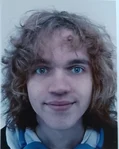
\includegraphics[width=\linewidth]{../img/magnus-profile.png}
\end{minipage}

\vspace{0.3cm}
\rule{\linewidth}{0.6pt}


% ---- TWO COLUMNS ----
\begin{minipage}[t]{0.44\textwidth}
\vspace{0pt}
\raggedright

\cvsection{Contact}
\begin{tabular}{@{}l l}
  Phone   & \Phone \\[2pt]
  Email   & \small\Email \\[2pt]
  Address & \Address \\[2pt]
  GitHub  & \href{https://\Github}{\Github} \\[2pt]
  Web     & \href{https://\Web}{\Web} \\
\end{tabular}

\cvsection{Education}
\textbf{2022 -- 2025}\\
Andreas Gordon Schule\\
\textit{Vocational school}

\vspace{0.3cm}

\textbf{August 2021}\\
Goetheschule Ilmenau

\cvsection{Skills}
\begin{itemize}
  \item Python | Django | Django REST Framework
  \item React | Next.js | TypeScript | Zustand | Tailwind CSS | ShadCN | Headless UI | Playwright | i18n
  \item PostgreSQL | TimescaleDB | Docker | Git | GitLab CI/CD
  \item SonarQube | Secure API design | SSH
  \item Responsive design | Accessibility (a11y) | WebSockets
  \item Intermediate Linux skills | Users/Groups | Filesystem | Logs | Updates/Patching | Process/Network inspection | 4 years daily driver
  \item AI tooling such as Claude Code and Codex
  \item Go | Gin | GORM | Ory | gRPC
  \item Rust (basics) | Axum | sqlx
  \item Java (beginner)
\end{itemize}

\cvsection{Languages}
\begin{itemize}
  \item German: Native
  \item English: Fluent
\end{itemize}

\end{minipage}
\hfill
\begin{minipage}[t]{0.52\textwidth}
\vspace{0pt}

\cvsection{Profile Summary}
\begin{itemize}
  \item Young, hands-on full-stack web developer from Thuringia with completed vocational training (best graduate, IHK South Thuringia 2025)
  \item Permanently employed at Sielaff GmbH \& Co.\ KG from August 2025 to January 2026
  \item Production-level experience with modern Python/Django backends and React/Next.js frontends, including Docker deployment
  \item Looking for new challenges in the Jena/Erfurt area or remote -- ideally full-stack, backend, or DevOps-related, but also open to focused UI development
\end{itemize}

\cvsection{Work Experience}

\textbf{Sielaff Software and Service GmbH \& Co.\ KG (Ilmenau)}
\hfill \textit{Aug 2025 -- Jan 2026}\\
Full-stack Web Developer
\begin{itemize}
  \item Further development, new development, and maintenance of internal web applications in an Industry 4.0 environment
  \item Full-stack responsibility: backend with Django/DRF, frontend with React/Next.js
  \item Containerization and deployment with Docker, including some GitLab CI/CD pipelines
  \item Real-time communication via WebSockets
  \item Database design and optimization
\end{itemize}

\vspace{0.35cm}

\textbf{Sielaff Software and Service GmbH \& Co.\ KG (Ilmenau)}
\hfill \textit{Late 2022 -- Mid 2025}\\
Apprenticeship as IT Specialist for Application Development
\begin{itemize}
  \item Three-year dual vocational training focused on full-stack web development
  \item Development of REST APIs, modern frontend interfaces, and internal automation tools
  \item Best graduate of IHK South Thuringia 2025
\end{itemize}

\end{minipage}

\end{document}
